% JuliaCon proceedings template
\documentclass{juliacon}
\usepackage{xspace}
\setcounter{page}{1}

\begin{document}

\newcommand{\chipsort}{{\tt ChipSort}\xspace}

% **************GENERATED FILE, DO NOT EDIT**************

\title{ChipSort: a SIMD and cache-aware sorting module}

\author[]{Nicolau Leal Werneck}
\affil[]{TomTom NV}

\keywords{Julia, Sorting, SIMD, Parallelism, Metaprogramming}



\maketitle

\begin{abstract}

Sorting is a fundamental programming problem with many important applications. While there are well-known sorting algorithms for conventional computers, special techniques are required to take the most out of real hardware offering features such as cache memory and instruction-level parallelism. ChipSort.jl is a Julia module for SIMD and cache-aware sorting. It implements sorting networks and bitonic merge networks with SIMD instructions, with configurable vector sizes. It also implements Combsort, which lends itself easily to vectorization and can achieve good performance depending on the memory access cost. Insertion sort is used to finalize. Large arrays are approached with a multi-way Mergesort. The implementation of ChipSort itself is of interest from a programming languages perspective due to its use of metaprogramming, more specifically Julia's generated functions. This enables custom code generation for different tasks and hardware at run-time, a feat owed to Julia. This article presents the implemented techniques as well as experiments that demonstrate speed gains compared to multiple standard libraries.

\end{abstract}

\section{Introduction}

Sorting has enjoyed an important place within computer programming topics for a long time. It has great importance to practical applications, being very useful to organize data for fast retrieval, and also attracts attention as a theoretically interesting problem in itself~\cite{DBLP:books/lib/Knuth98a}. While sorting is a well-understood problem in general, with a few classic algorithms available, achieving optimal performance for specific problems and architectures may require a careful algorithm selection rather than a simple parameter tuning \cite[Part II, Introduction]{DBLP:books/daglib/0023376}.

Many factors can influence the running time of a computer program, starting with algorithmic complexity and the base clock speed of the processor. The performance observed in real computers has been increasingly depending on processor features that are not taken into account by the simplest models, though. These features include cache memory and parallelism at the processor and instruction levels. Cache memory has become popular in consumer processors in the past couple of decades, and as long as memory access patterns exhibit temporal and spatial locality, it allows programs to attain a higher performance than would be possible with a simpler memory architecture~\cite[Chapter 3]{Drepper07whatevery}. Writing software with better support for parallelism has also become necessary to utilize the full potential offered by modern and future processors~\cite{wilson2018}.

One particular form of parallelism that concerns the present work are SIMD (single instruction, multiple data) instructions~\cite{SIMDtut}. This is a form of computation where a same operation is applied to different independent memory elements simultaneously. These operations can be described as operating over {\em vectors}, where each {\em lane} contains the same data that would be involved in carrying out the same operations as a scalar version of the same program. SIMD parallelism is only suitable to specific problems, and its use may imply in memory access constraints and even clock speed reductions. There are still cases where it can bring great performance while being conveniently employed.

The interest in sorting and the great relevance of cache memory and parallelism to modern computing have naturally led to research on sorting algorithms that account for these factors. Processors offering SIMD instructions and other forms of instruction-level parallelism started to become widely available in the early 2000s. One example is the introduction of SSE instructions in the x86 architecture~\cite[Chapter 1]{kusswurm18}. The current availability of processors with 512 bit registers underscores the necessity of being able to write software that utilizes vector operations, what can also benefit GPU programming.

At the time SIMD CPUs became widely available there was already a trend to employ specialized hardware like GPUs for scientific applications~\cite{larsen2001fast,DBLP:conf/micro/ThompsonHO02}. Although SIMD was used mostly for multimedia applications at first~\cite{CHEN2006509,DBLP:journals/mam/SlingerlandS05}, some early alternative uses include 3D graphics~\cite{DBLP:conf/pcm/MaY02} and machine learning~\cite{DBLP:conf/europar/StreyB01}.

Following earlier work on parallel sorting in other architectures, the late 2000s saw the first practical demonstrations of sorting with modern consumer SIMD chips~\cite{DBLP:conf/IEEEpact/InoueMKN07,DBLP:journals/pvldb/ChhuganiNLMHCBKD08}. Most of the techniques utilized then are still employed in more recent works~\cite{DBLP:journals/pvldb/BalkesenATO13,DBLP:journals/pvldb/InoueT15}.

This article presents {\tt ChipSort.jl}, a Julia module that implements SIMD and cache-aware sorting utilizing some of the techniques found in the literature. These include sorting and merging networks, the use of Combsort with Insertion sort finalization for medium sized arrays and of multi-way merging for large arrays. These techniques require not only tuning parameters such as vector and array sizes, but also generating specific code when implementing different size networks. \chipsort seeks to generate efficient custom code for each task, relying on Julia metaprogramming capabilities for that.

Section~\ref{sec:methods} ahead presents the techniques employed in \chipsort. Section~\ref{sec:experiments} presents experimental results assessing the performance of the module and Section~\ref{sec:conclusion} brings some concluding remarks.

\section{SIMD sorting techniques}
\label{sec:methods}
%
\chipsort offers four high-level functions that can be used in applications as replacements for other sorting functions such as {\tt sort} in the Julia standard library. The {\tt chipsort!} function does not require any configuration and offers a great performance on a wide range of cases. The remaining functions are suitable for arrays of specific size ranges, and require choosing some numeric parameters. The function {\tt chipsort\_large} offers a good overview of all the techniques implemented in the module, and this section is structured according to its stages. Some of these techniques may also be useful in other applications instead of sorting, one clear example being the in-place matrix transpose.

The way \chipsort  works mostly follows~\cite{DBLP:journals/pvldb/InoueT15}, although \chipsort does not support yet registers with key and payload. Another main difference is that Combsort is always employed with an Insertion sort finalization.

The function {\tt chipsort\_large} achieves sorting by first splitting the input array in chunks that are sorted separately with {\tt chipsort\_medium!}  and then merged simultaneously. This inner sort is performed in multiple steps:
\begin{enumerate}
\item sorting small blocks of data with a sorting network;
\item reordering vectors in memory according to a matrix transpose;
\item vectorized Combsort with a limited number of iterations;
\item regular insertion sort until the whole data is sorted.
\end{enumerate}

The remainder of this section details the multiple techniques employed in this process.

\subsection{Sorting networks}
%
Sorting networks~\cite[Sec. 5.3.4]{DBLP:books/lib/Knuth98a} are graphs composed by comparator modules, units that take two numbers in, and output the smallest and largest at specific outputs. By properly arranging comparators we can create a procedure to take an array of elements and output them in sequence. The design of a sorting network can minimize the total number of comparisons, or if they can be done in parallel, minimize the number of steps to complete the process.

A sorting network can be represented by a Knuth graph such as Figure~\ref{fig:sorting-network}. Each vertical line is a comparator. The graph represents a network that takes an array of four values $(A_1, A_2, A_3, A_4)$ and outputs the sorted sequence $(S_1, S_2, S_3, S_4)$.
\begin{figure}[htb]
\centerline{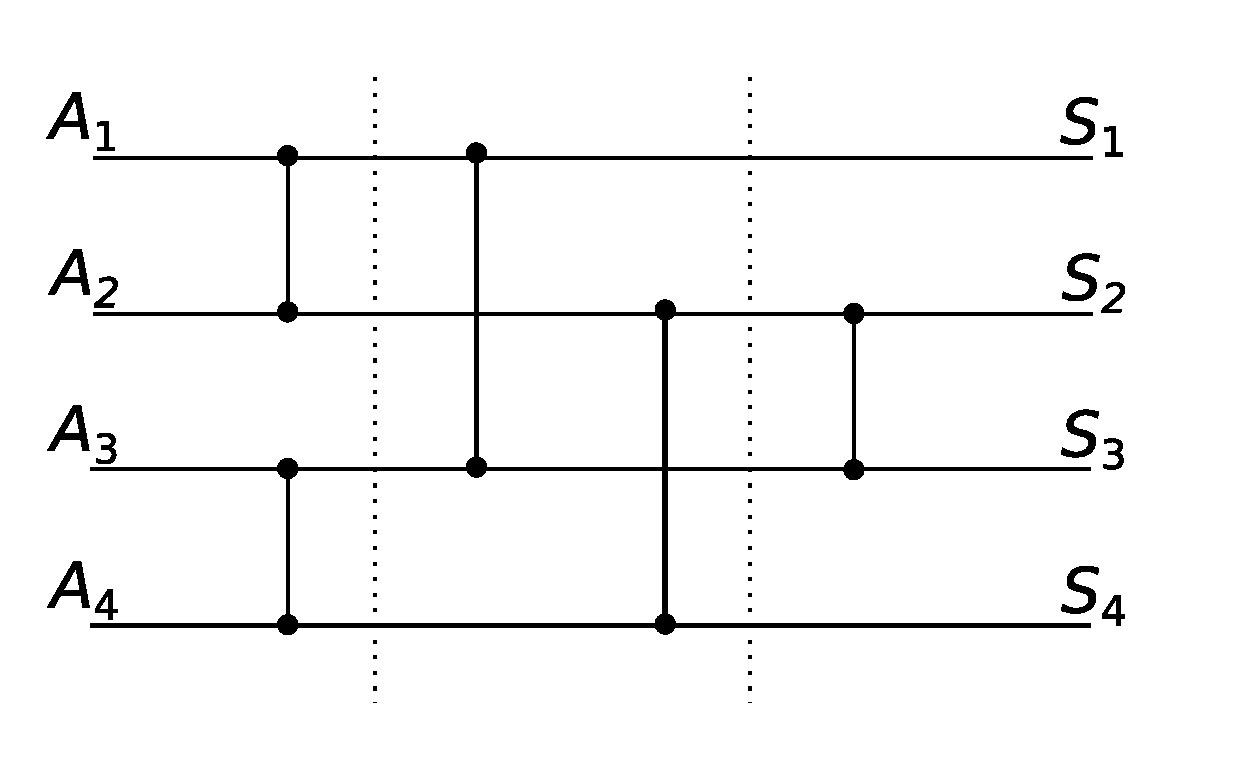
\includegraphics[width=0.6\linewidth]{fig/sorting-network-4.pdf}}
\caption{A sorting network for 4 elements. The dashed lines delimit each step where operations are independent of each other.}
\label{fig:sorting-network}
\end{figure}

In \chipsort, as in the related work, parallelism is mainly exploited by carrying out the comparisons of the sorting network over vectors of size $V$ contained in SIMD registers, effectively running $V$ networks simultaneously. Other forms of instruction-level parallelism can also be in play, though. It may be possible to parallelize instructions such as {\tt min} and {\tt max}, or the loading of data into registers. This is often done implicitly by the microarchitecture, and programmers can only make sure their code is suitable for this by properly ordering operations and avoiding branching, for instance. Part of this work is expected to be performed by the compiler, and in particular LLVM in the case of Julia.

\chipsort supports sorting networks of different sizes, currently only powers of 2, which are predefined as data structures in the file \href{https://github.com/nlw0/chipsort.jl/blob/d2d049b7413f0073476021fa62fb748803130768/src/sorting-network-parameters.jl}{\tt sorting-network-parameters.jl}. The generated function \href{https://github.com/nlw0/chipsort.jl/blob/d2d049b7413f0073476021fa62fb748803130768/src/sorting-networks.jl#L13}{\tt sort\_net} assigns each element of the sequence at each step to a variable, and the values from the next step are calculated according to the network specification. The comparisons are performed by the {\tt min} and {\tt max} functions, and the function is generic on the element types. Figure~\ref{fig:sort-net-listing} shows one example of generated code.

\begin{figure}[htb]
\begin{lstlisting}[language = Julia]
4 => (((1,2), (3,4)), ((1,3), (2,4)), ((2,3),))
\end{lstlisting}
\begin{lstlisting}[language = Julia]
input_0_1 = input[1]
input_0_2 = input[2]
input_0_3 = input[3]
input_0_4 = input[4]
input_1_1 = min(input_0_1, input_0_2)
input_1_2 = max(input_0_1, input_0_2)
input_1_3 = min(input_0_3, input_0_4)
input_1_4 = max(input_0_3, input_0_4)
input_2_1 = min(input_1_1, input_1_3)
input_2_3 = max(input_1_1, input_1_3)
input_2_2 = min(input_1_2, input_1_4)
input_2_4 = max(input_1_2, input_1_4)
input_3_1 = input_2_1
input_3_4 = input_2_4
input_3_2 = min(input_2_2, input_2_3)
input_3_3 = max(input_2_2, input_2_3)
return (input_3_1, input_3_2, input_3_3, input_3_4)
\end{lstlisting}
\caption{The parameters from a four-element sorting network consisting of three steps, and the corresponding code generated by {\tt sort\_net}.}
\label{fig:sort-net-listing}
\end{figure}

This function is a good first example of how \chipsort utilizes Julia's metaprogramming features. Multiple implementations of sorting networks are available in the literature~\cite{DBLP:journals/pvldb/ChhuganiNLMHCBKD08,sortingnetworksjl,ultrasort}, however they implement networks of different sizes straight as code. In \chipsort they are represented as data structures that guide a generated function to produce equivalent code. While this data structure is currently hard-coded, it could be potentially produced only when necessary by an algorithm such as Bose-Nelson, what remains a future plan for the module.

The {\tt sort\_net} generated function expects elements to which {\tt max} and {\tt min} are defined. It can be called with simple data types, {\em e.g.} {\tt sort\_net(4,2,5,3)} works. In practice \chipsort often calls this function with vectors, completely relying on {\tt SIMD.jl}~\cite{erik_schnetter_2019_2592633}. This module maps a vector in Julia similar to tuples or static arrays straight to LLVM vector types, ensuring SIMD code can be produced when possible and also allowing the flexibility of handling logic vectors that are larger than the actual registers, or spilling data to the stack if all registers are occupied.

\subsection{SIMD vectors transpose}
%
Consider a group of stacked SIMD vectors. Each column in this representation is termed a {\em lane}. The result from {\tt sort\_net} with vectors is that each lane contains a sorted sequence. This data must be transposed to produce sorted vectors. This is done in \chipsort through {\tt transpose\_vecs}, which is a generated function that supports rectangular matrices, but with dimensions constrained to powers of 2. The generated code consists mostly of calls to {\tt SIMD.shufflevec}. This is another instance of an operation that other projects~\cite{DBLP:journals/pvldb/BalkesenATO13,ultrasort} implement with multiple low-level functions contemplating each different case, while in \chipsort there is only a single Julia generated function that produces equivalent code.

Figure~\ref{fig:transpose-vecs} displays an example of 16 random integers loaded into SIMD registers as 4 vectors. After {\tt sort\_net} each lane contains a sorted sequence, and {\tt transpose\_vecs} turns the lanes into vectors (registers). The {\tt chipsort\_small!} function is essentially a sorting network followed by a transpose and a merge procedure.

\begin{figure}[htb]
\centerline{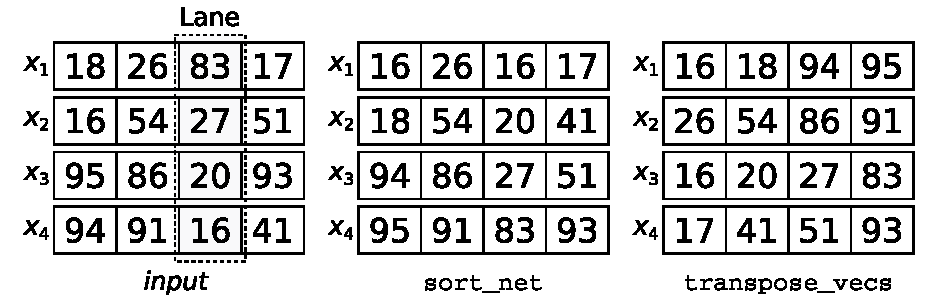
\includegraphics[width=0.99\linewidth]{fig/regs.pdf}}
\caption{Four vectors with four values, the result from a vectorized four-elements sorting network, and the transpose.}
\label{fig:transpose-vecs}
\end{figure}

\subsection{Bitonic Merge Networks}
%
A bitonic sequence starts either increasing or decreasing and contains at most one change of direction. Bitonic merge networks allow the creation of merge networks of different sizes, and they are again implemented in \chipsort with a single generated function, \href{https://github.com/nlw0/ChipSort.jl/blob/10eb1a962e720aee2bf8733c832468b51a782c1a/src/bitonic-merge-network.jl#L12}{\tt bitonic\_merge}. Merging two sorted vectors requires first reversing one of them, and the result is stored in two vectors containing the first and second halves of the complete sorted sequence.

Apart from the use in sorting small sequences and in the multi-way merge tree, bitonic merge networks can also be used to implement a regular merge sort. This technique was investigated in \chipsort only superficially, and while there were no promising results in terms of performance, \chipsort also contains the generated function {\tt bitonic\_merge\_interleaved} to illustrate how metaprogramming can help implement multiple simultaneous merges with interleaved execution, as done in other projects~\cite{DBLP:journals/pvldb/ChhuganiNLMHCBKD08}.

\subsection{Vectorized Combsort}
%
One of the most peculiar aspects of \chipsort, taken directly from AA-sort~\cite{DBLP:conf/IEEEpact/InoueMKN07,DBLP:journals/pvldb/InoueT15}, is the use of the Combsort algorithm. Combsort essentially generalizes Bubble sort in the same way that Shell sort generalizes Insertion sort~\cite{INCERPI198737,dobosiewicz1980efficient,Lacey:1991:FES:117187.117218,DBLP:books/lib/Knuth98a,DBLP:books/daglib/0023376}. The array is swept multiple times, ordering pairs of values at a given distance from each other. The distance is reduced each time by $\frac{4}{3}$. Parallelism is achieved either by parallelizing the operations from a single array or by processing independent arrays of the same size.

\chipsort contains two functions that utilize Combsort, employing these two distinct forms of parallelism. The first is {\tt chipsort!}, a serial implementation of the algorithm which is vectorized implicitly by the optimizing compiler. {\tt chipsort!} starts with Combsort until the interval size is 1, when it switches to Insertion sort.

The other function is {\tt chipsort\_medium!}, an explicitly vectorized implementation utilizing {\tt SIMD.jl}. This second function also performs a number of operations before and after Combsort. It consists of the following steps:
\begin{enumerate}
\item Apply a sorting network on $K$ blocks of $J$ vectors of size $V$.
\item Vectorized Combsort until the interval size is 1.
\item Transpose blocks.
\item Transpose data in-place from $K$ blocks of $J$ vectors into $J$ blocks of $K$ vectors.
\item Vectorized Combsort again.
\item Sort blocks again.
\item Insertion sort.
\end{enumerate}

After the first two steps the result is essentially a matrix where the $K\times J$ columns are the vectors, and each of the $V$ rows contains an approximately sorted sequence. The transpose steps reshape each row into a new block. Each row is processed independently at first, and the transpose allows elements from distinct groups to interact. The last step is necessary to ensure the whole array is sorted, not viewed anymore as a matrix with independent rows.

In both implementations switching to Insertion sort presents a better performance than sticking to Combsort until the end. Once the interval becomes 1 Combsort essentially becomes Bubble sort, thus finding an alternative seems beneficial. Insertion sort should fare well because the array is now approximately sorted, and any out-of-order elements should be already close to their destinations.

Finishing a sorting method with Insertion sort is a common practice, present at least in Musser's Introsort~\cite{musser1997introspective}. This is also akin to the classic method used in the Julia standard library, switching to Insertion sort when the array becomes too small. The difference is that Combsort is not a divide-and-conquer approach, and therefore Insertion sort must be applied once on the whole array.

The utilization of Insertion sort as a final stage to Combsort has been considered before~\cite{combwiki,INCERPI198737}, and Insertion sort was even employed by~\cite{DBLP:journals/pvldb/InoueT15} for dealing with partial keys. The main contribution of the present work may be to extend AA-sort~\cite{DBLP:conf/IEEEpact/InoueMKN07,DBLP:journals/pvldb/InoueT15} by giving a larger role to Insertion sort and also relying more on automatic vectorization by the compiler.

\subsection{In-place matrix transpose}
%
In-place matrix transposition can be attained by moving a number to its destination, then moving away the number that was found there, and so on, until a cycle is completed and a new number is selected to be moved~\cite{10.1093/comjnl/2.1.47}. While carrying out this procedure is simple, it is not trivial to find out what are the cycles to transpose a matrix of any given dimensions, and even finding out the number of cycles turns out to be a difficult problem~\cite[1.3.3-12]{DBLP:books/lib/Knuth97}.

\chipsort contains the generated function \href{https://github.com/nlw0/ChipSort.jl/blob/10eb1a962e720aee2bf8733c832468b51a782c1a/src/transpose-vecs.jl#L19}{\tt transpose!} to perform in-place matrix transposition. The cycle seeds are computed at the time of code generation, and at run-time the function only moves the data, computing the index sequences and detecting when each cycle finishes. Therefore even though the function is completely generic, supporting any shape, the most complex part of the problem is tackled programmatically during code generation, resulting in a very simple run-time code.

\subsection{Vectorized multi-way merging}
%
Merging multiple arrays simultaneously requires the creation of a {\em merge tree} to keep some intermediate data. Each node in this tree is essentially an iterator traversing the merger of two arrays in the lower level. To employ the vectorized bitonic merge network in this process it is necessary to keep a whole vector at each node of the tree. To produce the next vector of elements one of the two source arrays is selected according to their smallest next element, and a whole vector is pulled from that array. This vector is merged with the intermediate one, and the first half of the resulting sequence can be taken to the next level of the tree, while the second half is kept as the new intermediate data.

Given a set of sorted arrays, once the tree is initialized data is taken from it one vector at a time, producing the final sorted sequence. Each time a new vector is requested the tree is traversed following the smallest element among the node children, until one of the input arrays is reached. The data from the array is then loaded from memory and merged with the intermediate data, producing new updates moving through the tree until the root is reached.

The intermediate data from the tree is kept by \chipsort in a contiguous array, treated as a heap. Assuming 1-based indexing, each node ancestor can be simply found by the Euclidean division of its index by 2. This data is assumed to fit some level of cache memory during operation, as in the related work~\cite{DBLP:conf/IEEEpact/InoueMKN07,DBLP:journals/pvldb/ChhuganiNLMHCBKD08,DBLP:journals/pvldb/InoueT15}.


\section{Experiments}
\label{sec:experiments}
%
This section reports experiments with the \chipsort methods, as well as alternative ones. The term {\it method} can be understood as both the algorithms and their implementations in the Julia language. The specific methods tested were:
\begin{itemize}
\item {\tt chipsort!} Combsort finishing with Insertion sort, written as a serial program and vectorized by the compiler.
\item {\tt chipsort\_small!} in-register, based on sorting networks.
\item {\tt chipsort\_medium!} vectorized Combsort, plus additional steps, finishing with Insertion sort.
\item {\tt chipsort\_large} merge-sort with a multi-way merge tree, starting from chunks processed by {\tt chipsort\_medium!}.
\item {\tt insertion\_sort!} Insertion sort taken from the Julia library.
\item {\tt sort!} the Julia standard sort, Quicksort finishing with Insertion sort for small arrays (\href{https://github.com/JuliaLang/julia/blob/de3401908a506727ed70b3e953bd721ab4d66109/base/sort.jl#L461}{20} elements).
\end{itemize}

The {\tt !} implies in-place operation. The allocation time for {\tt chipsort\_large} was not discounted in our analyses.

\subsection{Small arrays}
In our first experiment we evaluate the sorting of small arrays, with 64 32-bit values. The {\tt chipsort\_small!} method based on sorting and bitonic merge networks was compared to serial Insertion sort, the Julia sort and {\tt chipsort!}. The short running time makes it challenging to perform proper measurements, therefore the task was to sort 128 sequences of 64 contiguous values in memory, forming a single block of $2^{13}$ uniform random entries. Sorting was performed in-place, in a for-loop. The results are in Table~\ref{tab:bench-small}.

\begin{table}[h]
\tabcolsep22pt
\tbl{Sorting $128 \times 64$ {\tt UInt32} elements.}{
\begin{tabular}{|l|r|}\hline
Method & Median time\\\hline
{\tt chipsort\_small!} & 57.206 $\mu$s\\\hline
{\tt chipsort!} & 133.510 $\mu$s\\\hline
Insertion sort & 194.679 $\mu$s\\\hline
Julia standard & 222.910 $\mu$s\\\hline
\end{tabular}}
\label{tab:bench-small}
\end{table}

The {\tt chipsort\_small} function achieved a significant acceleration of over 3 times relative to Insertion sort or the Julia standard function, and twice over {\tt chipsort!}. Even though the in-register function was clearly faster, this first experiment already demonstrates the potential of {\tt chipsort!}, which presented a speedup of at least 46\% compared to the other alternatives.

\subsection{Medium and large arrays}
Our second experiment compared many different methods on inputs of exponentially increasing sizes, from $2^6$ to $2^{20}$. Figure~\ref{fig:bench-time} displays the resulting measurements. Although the curves look too concentrated in this visualization, it is possible to notice that {\tt chipsort!} consistently outperforms the Julia standard library by a factor of 80\% to 100\%, or up to twice as fast. We can also observe that Insertion sort soon becomes too inefficient.

\begin{figure}[htb]
\centerline{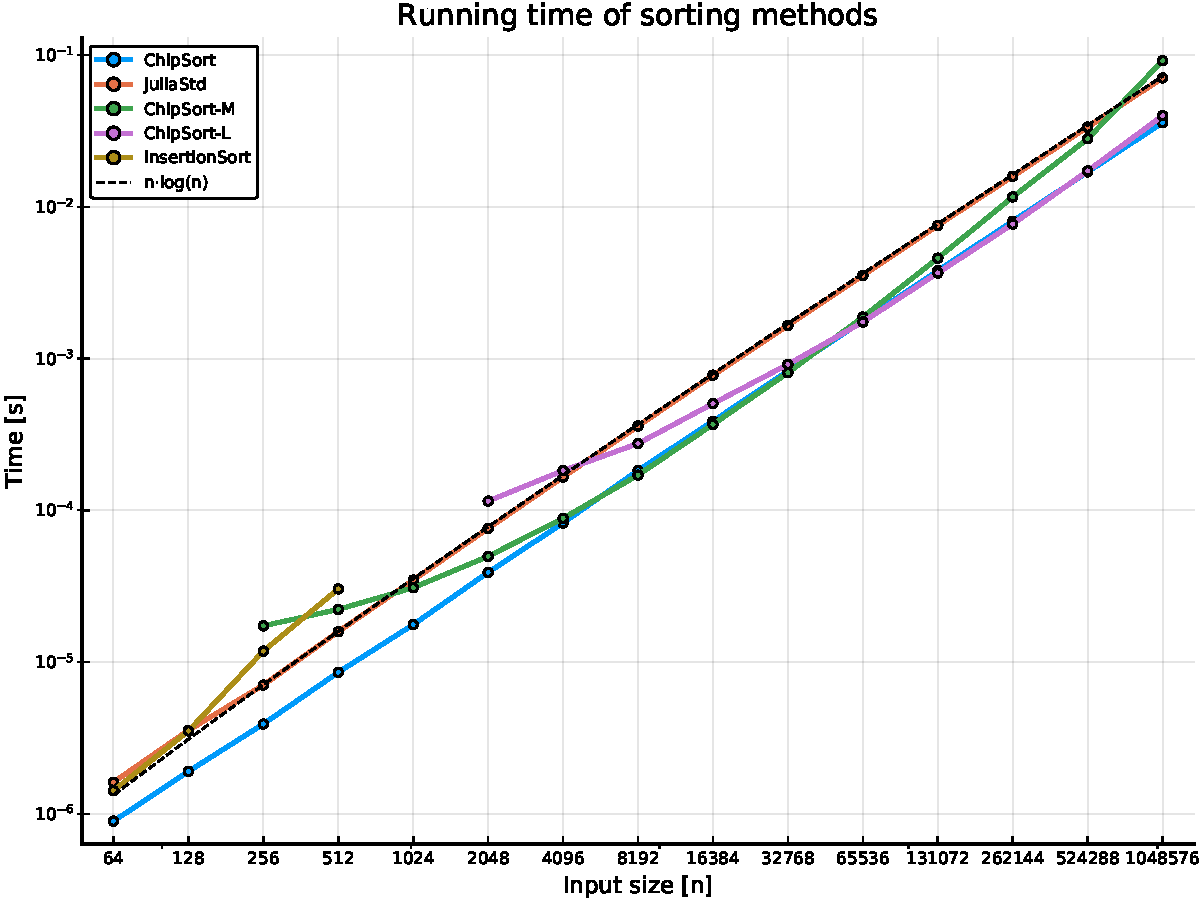
\includegraphics[width=\linewidth]{fig/chipsort-bench-time.pdf}}
\caption{Running time of the different sorting methods studied.}
\label{fig:bench-time}
\end{figure}

Figure~\ref{fig:bench-curves} shows a different visualization from the same data with the time divided by the input size. The vertical dotted lines indicate the size of each cache level. Here we can see more clearly how {\tt chipsort\_medium!} and {\tt chipsort\_large} slightly outperform {\tt chipsort!} in a few cases.

\begin{figure}[htb]
\centerline{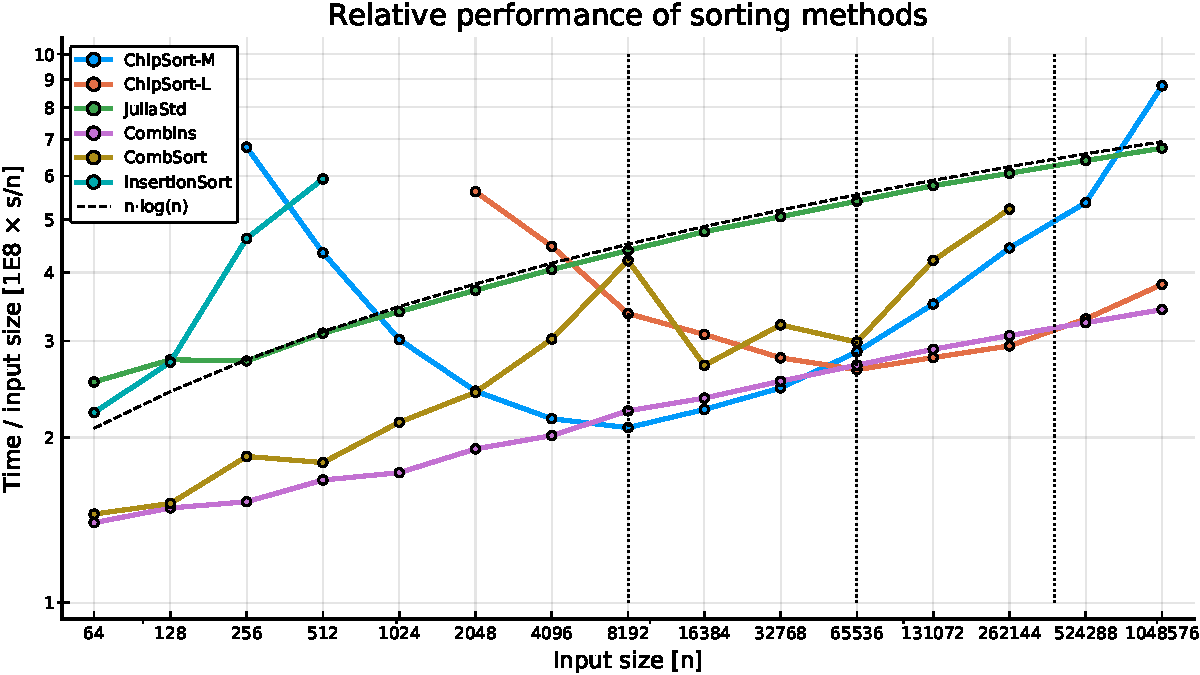
\includegraphics[width=\linewidth]{fig/chipsort-bench-curves.pdf}}
\caption{Curves displaying the relative running time from each studied method. The ordinate represents the median of the measured running times divided by the input size at each test. Lower is faster.}
\label{fig:bench-curves}
\end{figure}

Figure~\ref{fig:bench-cdf} displays the measured times for $2^{13}$ and $2^{18}$ elements. All the tested \chipsort methods surpass the Julia standard library in these cases. In the $2^{13}$ case {\tt chipsort\_medium!} exhibits a slight speedup of 7.3\% over {\tt chipsort!}, and on the $2^{13}$ case it is {\tt chipsort\_large!} with 4.4\%.

\begin{figure*}[htb]
  \centerline{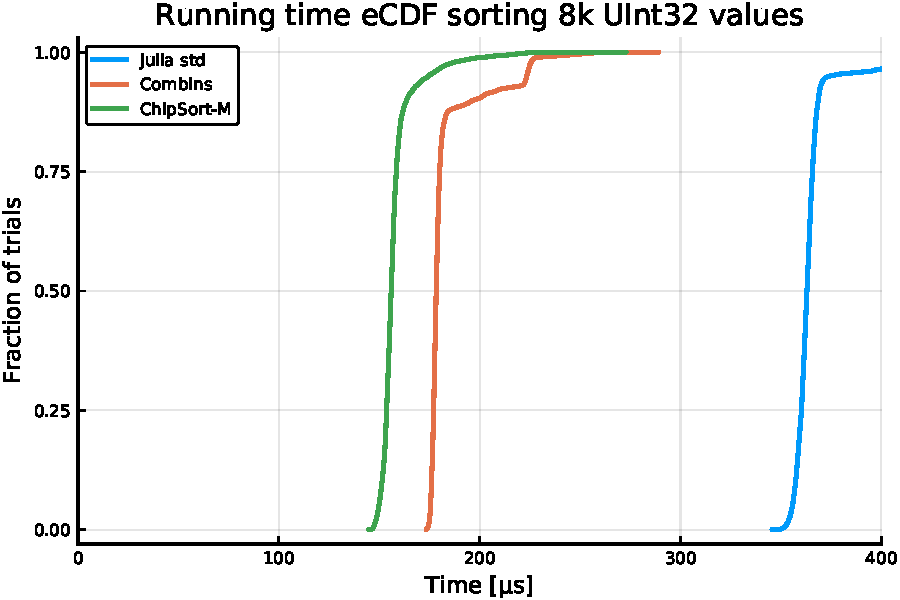
\includegraphics[width=0.4\linewidth]{fig/chipsort-bench-8k.pdf}
    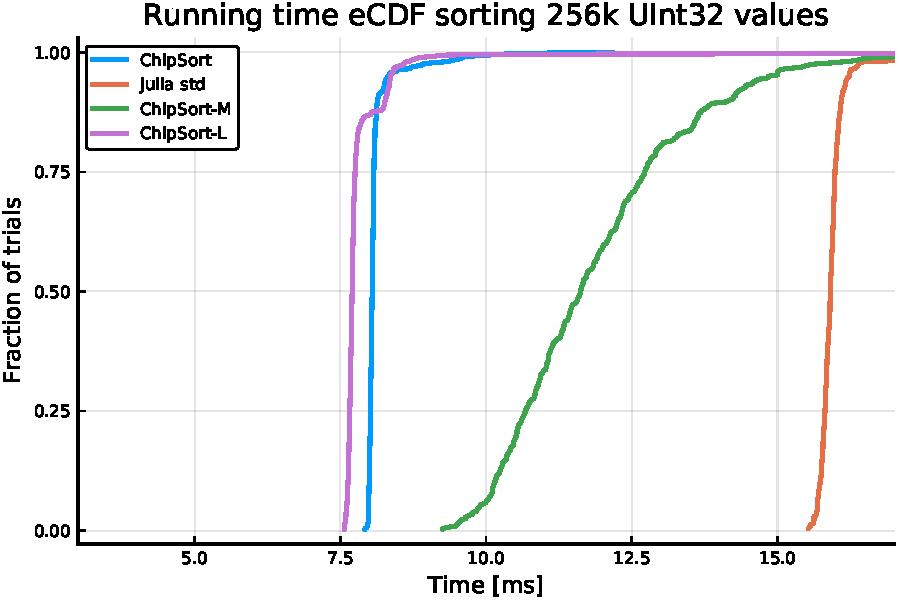
\includegraphics[width=0.4\linewidth]{fig/chipsort-bench-256k.pdf}}
\caption{Empirical CDF from different methods with 8k and 256k {\tt UInt32} values. Results from 10,000 measurements.}
\label{fig:bench-cdf}
\end{figure*}

\subsection{Other platforms}
One last experiment was carried out with different programming languages in the same machine and with Julia in different machines, to provide more context. Table~\ref{tab:bench-cxx} displays statistics collected from Julia, Python and C++ programs. Versions utilized were Julia 1.3.0-DEV.431, Python 3.6.8 with Numpy 1.14.3 and GCC 8.3.0 with libstdc++ 6.0.25 on a Ubuntu 18.04 system. For the case of Python the measurements obtained by calling the function through PyCall were better than using the native Python shell, therefore the best value was kept. Results obtained for C++ with Julia inter-operation using {\tt Cxx.jl} were slightly worse than native, thus discarded. While Numpy was almost as fast as Julia, no reason could be found for the dismal performance of the C++ standard library.

\begin{table}[h]
\tabcolsep11pt
\tbl{Sorting arrays of 8k and 1M {\tt UInt32} elements in different software platforms.}{
\begin{tabular}{|l|r|r|}\hline
Method & 8k & 1M\\\hline
\chipsort & 172.35 $\mu$s & 35.28 ms\\\hline
Julia standard & 337.03 $\mu$s & 68.39 ms\\\hline
Numpy via PyCall & 354.55 $\mu$s & 70.01 ms\\\hline
C++ {\tt std::qsort} & 770.93 $\mu$s & 143.48 ms\\\hline
C++ {\tt std::sort} & 1,177.54 $\mu$s & 221.27 ms\\\hline
\end{tabular}}
\label{tab:bench-cxx}
\end{table}

Table~\ref{tab:bench-512} contains the results for {\tt chipsort!} and the Julia standard {\tt sort!} on an Intel processor with AVX512 instructions, and an ARM processor with 128-bit NEON instructions.
\begin{table}[h]
\tabcolsep11pt
\tbl{Sorting arrays of 8k and 1M {\tt UInt32} elements in different hardware platforms.}{
\begin{tabular}{|l|l|r|r|}\hline
Chip & Method & 8k & 1M\\\hline
AXV512 & \chipsort & 177.4 $\mu$s & 35.20 ms\\\hline
AXV512 & Julia standard & 347.5 $\mu$s & 69.07 ms\\\hline
NEON & \chipsort & 350.9 $\mu$s & 73.36 ms\\\hline
NEON & Julia standard & 573.2 $\mu$s & 113.68 ms\\\hline
\end{tabular}}
\label{tab:bench-512}
\end{table}
No change in performance can be seen on the AVX512 machine, and on the ARM machine the speedup was smaller than before: only 60\%. The most notable fact in this experiment is that the same high-level and serial code successfully produced a vectorized sort on machines with different vector sizes and even instruction sets, always with a beneficial outcome.

\section{Conclusion}
\label{sec:conclusion}
%
We have presented \chipsort, a Julia module for SIMD and cache-aware sorting. The main sorting method utilized in \chipsort is Combsort finalized with Insertion sort. This method is based on previous proposals for SIMD sorting~\cite{DBLP:conf/IEEEpact/InoueMKN07,DBLP:journals/pvldb/InoueT15} and other practical sorting methods~\cite{INCERPI198737,musser1997introspective}. This method was implemented as a serial program vectorized by the Julia compiler and LLVM, resulting in a sorting function up to twice as fast as the Julia standard library sort. This performance holds for at least a million 32-bit integers in a personal computer.

Other techniques available in \chipsort are sorting networks, bitonic merge networks, in-place matrix transpose and a multi-way merge tree. Vectorized in-register sorting, although limited to small powers of 2, proved to deliver speedups of up to 3 times relative to the standard library.

Results were limited for the method dedicated to large arrays, only narrowly surpassing the main \chipsort method in few cases. Merge-based techniques may be more advantageous when sorting large records, though.

While the main \chipsort method relies on compiler optimizations, other methods utilize explicit vectorization trough {\tt SIMD.jl}. \chipsort makes extensive use of metaprogramming, more specifically Julia generated functions. This allows functions like sorting networks to be implemented in an abstract and generic way. The networks are represented as data structures, used by a higher-level program to assemble the final network code. This contrasts with other libraries where different networks are implemented straight as final functions. Julia also has the opportunity to perform custom optimizations since \chipsort is implemented in pure Julia with abstract methods that can be specialized.

It is a testament to the quality of the Julia compiler infrastructure that the most successful method implemented in \chipsort has no explicit vectorization or intrinsics. It is just a simple, scalar implementation of Combsort that is optimized by the compiler to generate code adapted to different problem settings and to the hardware architecture at run-time. And in the cases where explicit vectorization is necessary Julia still offers a suitable framework that allowed \chipsort to implement sophisticated techniques with concise code. This project can illustrate how well Julia implements traditional language features such as parametric types, and its metaprogramming features make it stand out from other languages even more.

Some future prospects for \chipsort are to implement missing features such as buffers in the merge tree and stable sorting of key-payload data; explore the limits of in-register processing in modern 512-bit architectures an eventually GPUs; explore how to interact with the compiler in order to optimize code for complex tasks such as multi-stage multi-threaded merge-sorting of large arrays.




\input{bib.tex}

\end{document}

% Inspired by the International Journal of Computer Applications template

% latexmk -bibtex -pdf paper.tex
